\documentclass[•]{article}
\usepackage{graphicx}
\usepackage{float}


\begin{document}
\title{Heat and Mass Week 2}
\maketitle
\section*{Multilayer Plane Walls}
The system can be made more complicated by putting two materials with different thermal conductivity in contact, and trying to solve the solution of the system as before. This can be seen below in figure 1.\\

The system is solvable, as at the interface of the two materials, the heat flux and temperature should be equivalent. This assumes the system is at steady state. The differential equations must be solved seperately for both materials, and the temperature profile as a function of x is going to be discontinuous at the boundary of the two materials.

\begin{figure}[H]
\begin{center}
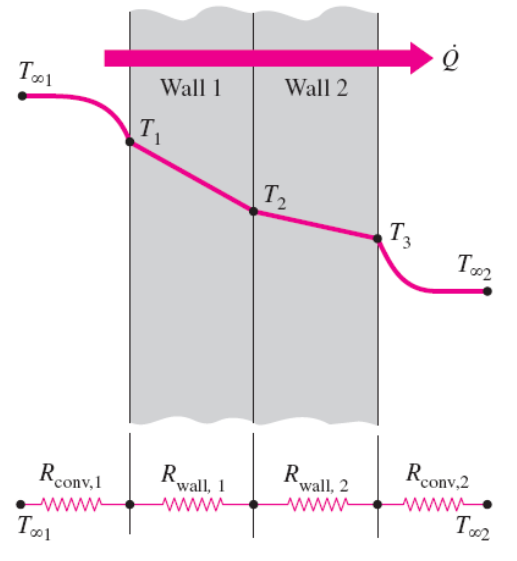
\includegraphics[scale=0.4]{TwoWall.png}
\end{center}
\caption{An image illustrating the ideal multilayer plane wall}
\end{figure}

One of the methods of modelling the temperature profile through the solid is calculating the equivalent thermal resistance of the different walls in series, using that to find the $\dot{Q}$ through the solid, and then further using that to calculate the temperature profile. In an analogy to circuits, the heat flux($\dot{Q}$) is current, and the temperature drop is voltage. 

\section*{Split Plane Walls}
One of the problems that may occur, is one in which the plane wall is split between two materials perpendicular to the direction of the heat flow. In order to solve these problems, it is assumed that the interface between the two plane walls is insulated, and that there is only heat flow in one direction (left to right in this instance).\\

In the analogy to circuits, the two walls can be modelled as resistors in parallel, and it's reduced to a circuits problem.
\begin{figure}[H]
\begin{center}
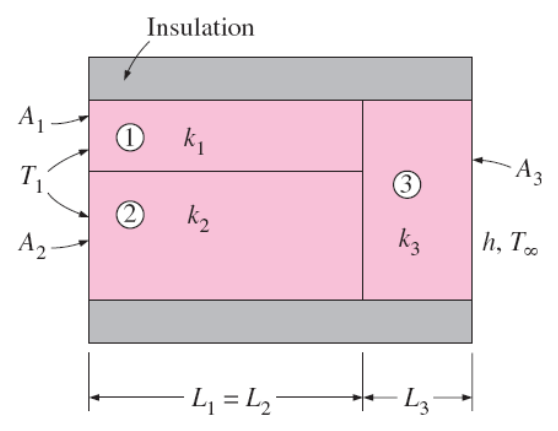
\includegraphics[scale=0.4]{SplitWall.png}
\end{center}
\caption{An image illustrating two walls are in contact parallel to the direction of heat flow}
\end{figure}

\section*{Spherical Walls}
In the event of a spherical coordinate system, the equivalent resistance can be slightly harder to calculate.

\begin{figure}[H]
\begin{center}
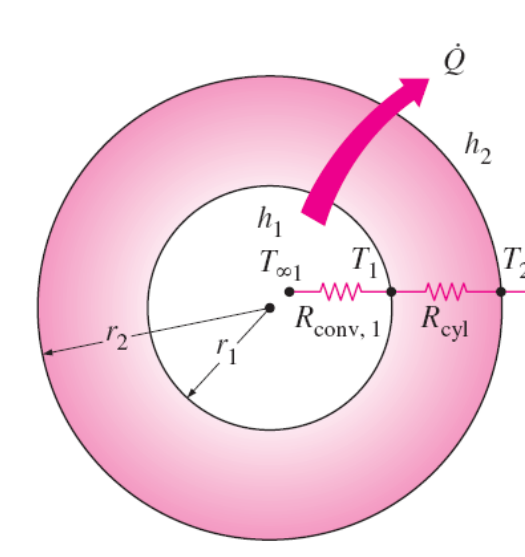
\includegraphics[scale=0.4]{SphericalWall.png}
\end{center}
\caption{An image illustrating walls that completely enclose a sphere of some fluid}
\end{figure}

\end{document}